% !TeX root = ../main.tex

\section{Baseline: Kaiming Initialization Study}
\label{sec:relu1-kaiming}

\subsection*{Experimental Setup}
Fifty independent training runs of the two-ReLU model were launched with
\emph{Kaiming-normal} weights, bias $0$, Adam
($lr=0.01$, $\beta=(0.9,0.99)$) and a hard cap of $800$ epochs.
Training stopped under either of two conditions:
\begin{enumerate*}[label=(\roman*)]
    \item \textbf{Convergence} - loss fails to improve by
          $10^{-24}$ for ten consecutive epochs
          (e.g.\ epoch 367 in one run);
    \item \textbf{Accuracy threshold} - mean-squared error
          $\mathcal L\le10^{-7}$ (e.g.\ epoch 247).
\end{enumerate*}
All further chapters inherit this protocol unless stated otherwise.

% ------------------------------------------------------------------
\subsection*{Classification Accuracy}

\begin{table}[h]
\centering
\caption{Final accuracy counts over $50$ runs.}
\label{tab:relu1-kaiming-accuracy}
\begin{tabular}{lccccc}
\toprule
Accuracy & 0\,\% & 25\,\% & 50\,\% & 75\,\% & 100\,\% \\ \midrule
Runs & 0 & 0 & 0 & 26 & 24 \\ \bottomrule
\end{tabular}
\end{table}

\textbf{Observation}  
Bare Kaiming succeeds \emph{less than half} the time; the rest stall at
$75\,\%$ (three of four XOR points correct).

% ------------------------------------------------------------------
\subsection*{Convergence Timing}

\begin{table}[h]
\centering
\caption{Epochs to early-stop (percentiles over successful runs).}
\label{tab:relu1-kaiming-epochs}
\begin{tabular}{lccccc}
\toprule
Percentile & 0\,\% & 25\,\% & 50\,\% & 75\,\% & 100\,\% \\ \midrule
Epochs & 32 & 98 & 164 & 242 & 368 \\ \bottomrule
\end{tabular}
\end{table}

The spread spans an order of magnitude, hinting at widely differing
initial geometries.

% ------------------------------------------------------------------
\subsection*{Final Loss Distribution}

Two tight clusters emerge:
\begin{itemize}
  \item $\mathbf{24}$ successful runs finish near
        $\mathcal L\!\approx\!10^{-8}$,
  \item $\mathbf{26}$ stalled runs concentrate at
        $\mathcal L\!\approx\!2.5\times10^{-1}$.
\end{itemize}
No run terminates in intermediate territory, reflecting the discrete
accuracy split of Table~\ref{tab:relu1-kaiming-accuracy}.

% ------------------------------------------------------------------
\subsection*{Hyperplane Geometry}
\label{sec:relu1-hyperplane-geometry}

We replicate the two geometric analyses from
Section~\ref{sec:abs1-init}:

\begin{enumerate}[label=(G\arabic*)]
    \item \textbf{Distance-pattern clustering} –  
          Each run yields the pair
          $(d_{0},d_{1})$ of mean distances from the hyperplane~$f(x)=0$
          to the \textbf{False} and \textbf{True} inputs.
          DBSCAN ($\varepsilon=0.2$) discovers \textbf{three} clusters:  
          one dominant group matching the prototype-surface prediction
          $(0,\sqrt2)$ and two looser satellites produced by the runs that
          stalled at $75\,\%$.
    \item \textbf{Weight-space clustering} –  
          Clustering the parameter quadruples
          $(w^{(0)},b^{(0)},w^{(1)},b^{(1)})$
          with $\varepsilon=0.2$ returns
          nine small clusters plus ten singleton “noise” points.
          Although less tight than in Abs1, the two largest clusters are
          near-mirror centroids, echoing the
          $|z|=\operatorname{relu}(z)+\operatorname{relu}(-z)$ identity.
\end{enumerate}

\begin{figure}[h]
  \centering
  \begin{subfigure}{0.30\textwidth}
    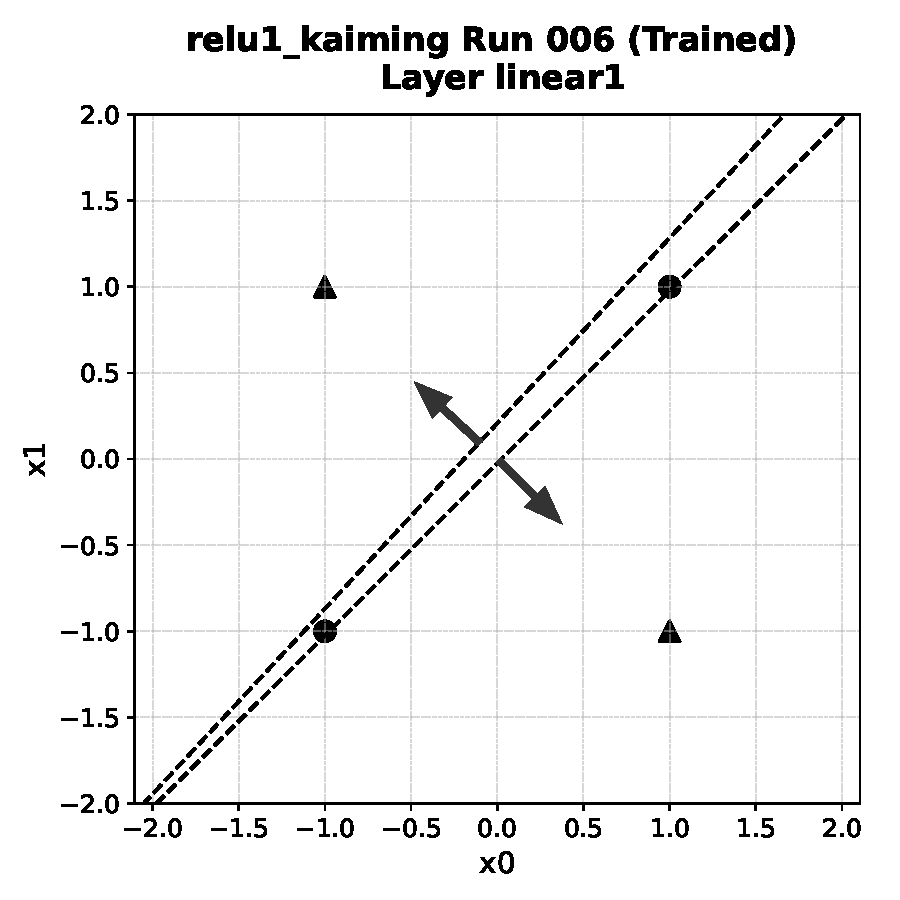
\includegraphics[width=\linewidth]{relu1/figs/success_mirror.pdf}
    \caption{Run 006 (success)}
  \end{subfigure}\hfill
  \begin{subfigure}{0.30\textwidth}
    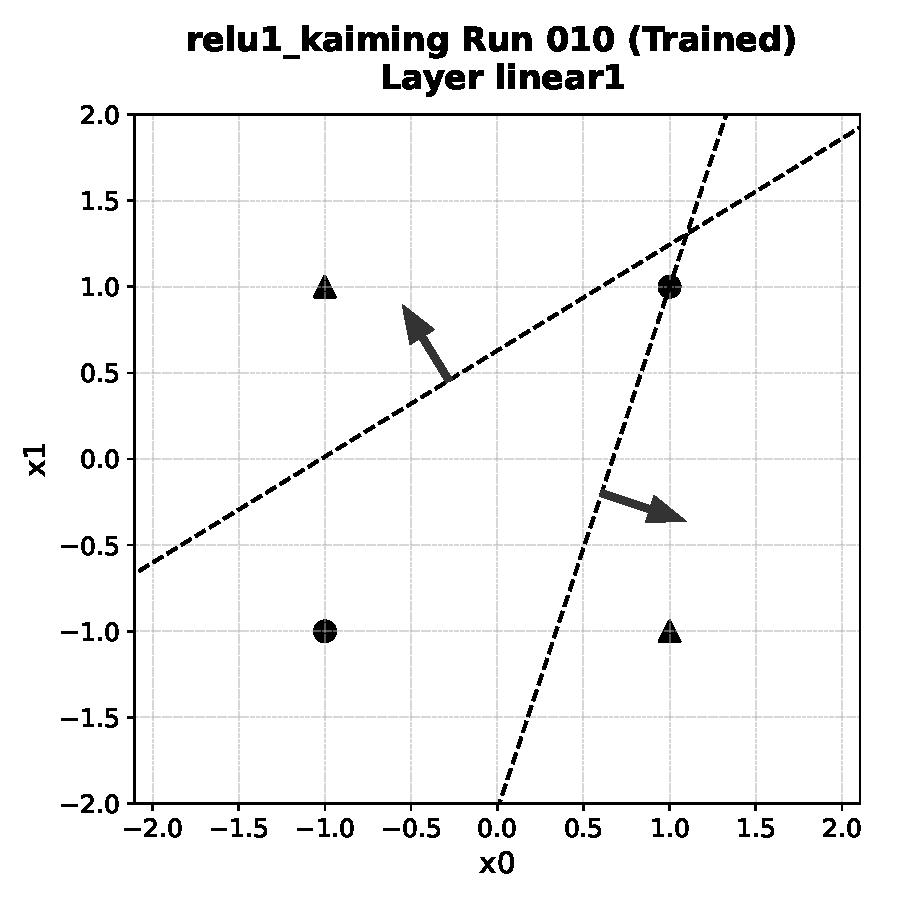
\includegraphics[width=\linewidth]{relu1/figs/success_no_mirror.pdf}
    \caption{Run 019 (initial)}
  \end{subfigure}\hfill
  \caption{Representative hyperplanes.  Dashed lines: $f_k(x)=0$ for each
           neuron; arrows show normal directions.  \(\bullet\): class-0,
           \(\blacktriangle\): class-1.}
  \label{fig:relu1-kaiming-planes}
\end{figure}

\paragraph{Interpretation}
Figure~\ref{fig:relu1-kaiming-planes} illustrates two 100\% accuracy results. Run 006 converges to the anticipated pair of almost-mirror hyperplanes, while Run 010 uses the leeway afforded by ReLU to learn hyperplanes oriented about 50 degrees from each other.

% ------------------------------------------------------------------
\subsection*{Activation Coverage Snapshot}

Across all 50 runs, \textbf{39} begin with at least one XOR point inactive (\(\operatorname{relu}(z)=0\) for both neurons). 
Among these, 14 still reach 100\,\% accuracy, showing that dead inputs \emph{can} revive but not invariably.
This statistic motivates the detection and re-initialisation tactics explored in Section~\ref{sec:relu1-reinit}.

% ------------------------------------------------------------------
\paragraph{Discussion}
\begin{itemize}
  \item Bare Kaiming achieves perfect XOR only \textbf{48\,\%} of the time.
  \item Successful runs agree with prototype-surface theory-two sign-symmetric
        distance patterns-but the clusters are fuzzier than in Abs1 because
        the ReLU's inactive half-space allows more slack.
  \item The prevalence of early dead inputs and the bimodal loss histogram
        make Kaiming an ideal baseline for testing activation variants,
        re-initialisation rules, and runtime monitors in the sections that
        follow.
\end{itemize}

\hrulefill
